\begin{frame}{Results}
\begin{block}{Results Organization}
	\begin{enumerate}
		\item Simulation results: Open loop (model equivalence)
		\item Experimental results: Tracking control
		
	\end{enumerate}
\end{block}
\end{frame}

%%%%%%%%%%%%%%%%%%%%%%%%%%%%%%%% FRAME %%%%%%%%%%%%%%%%%%%%%%%%%%%%%%%%
\begin{frame}{Openloop Simulation}
Nonlinear error system and TS-fuzzy error system were subjected to the same input signal
\begin{equation}
u = \begin{bmatrix}
\sin(t)+\sin(1.3t)\\
-\cos(4t)-\cos(5.3t)\\
\sin(2t)+\sin(2.3t)\\
\cos(0.5t)+cos(0.3t)
\end{bmatrix}
\end{equation}
\end{frame}

\begin{frame}
\begin{figure}[!htb]
	% \includegraphics[trim={5cm 0 0 0},clip]{example-image-a}
	% 	 trim={<left> <lower> <right> <upper>}
	\centering
	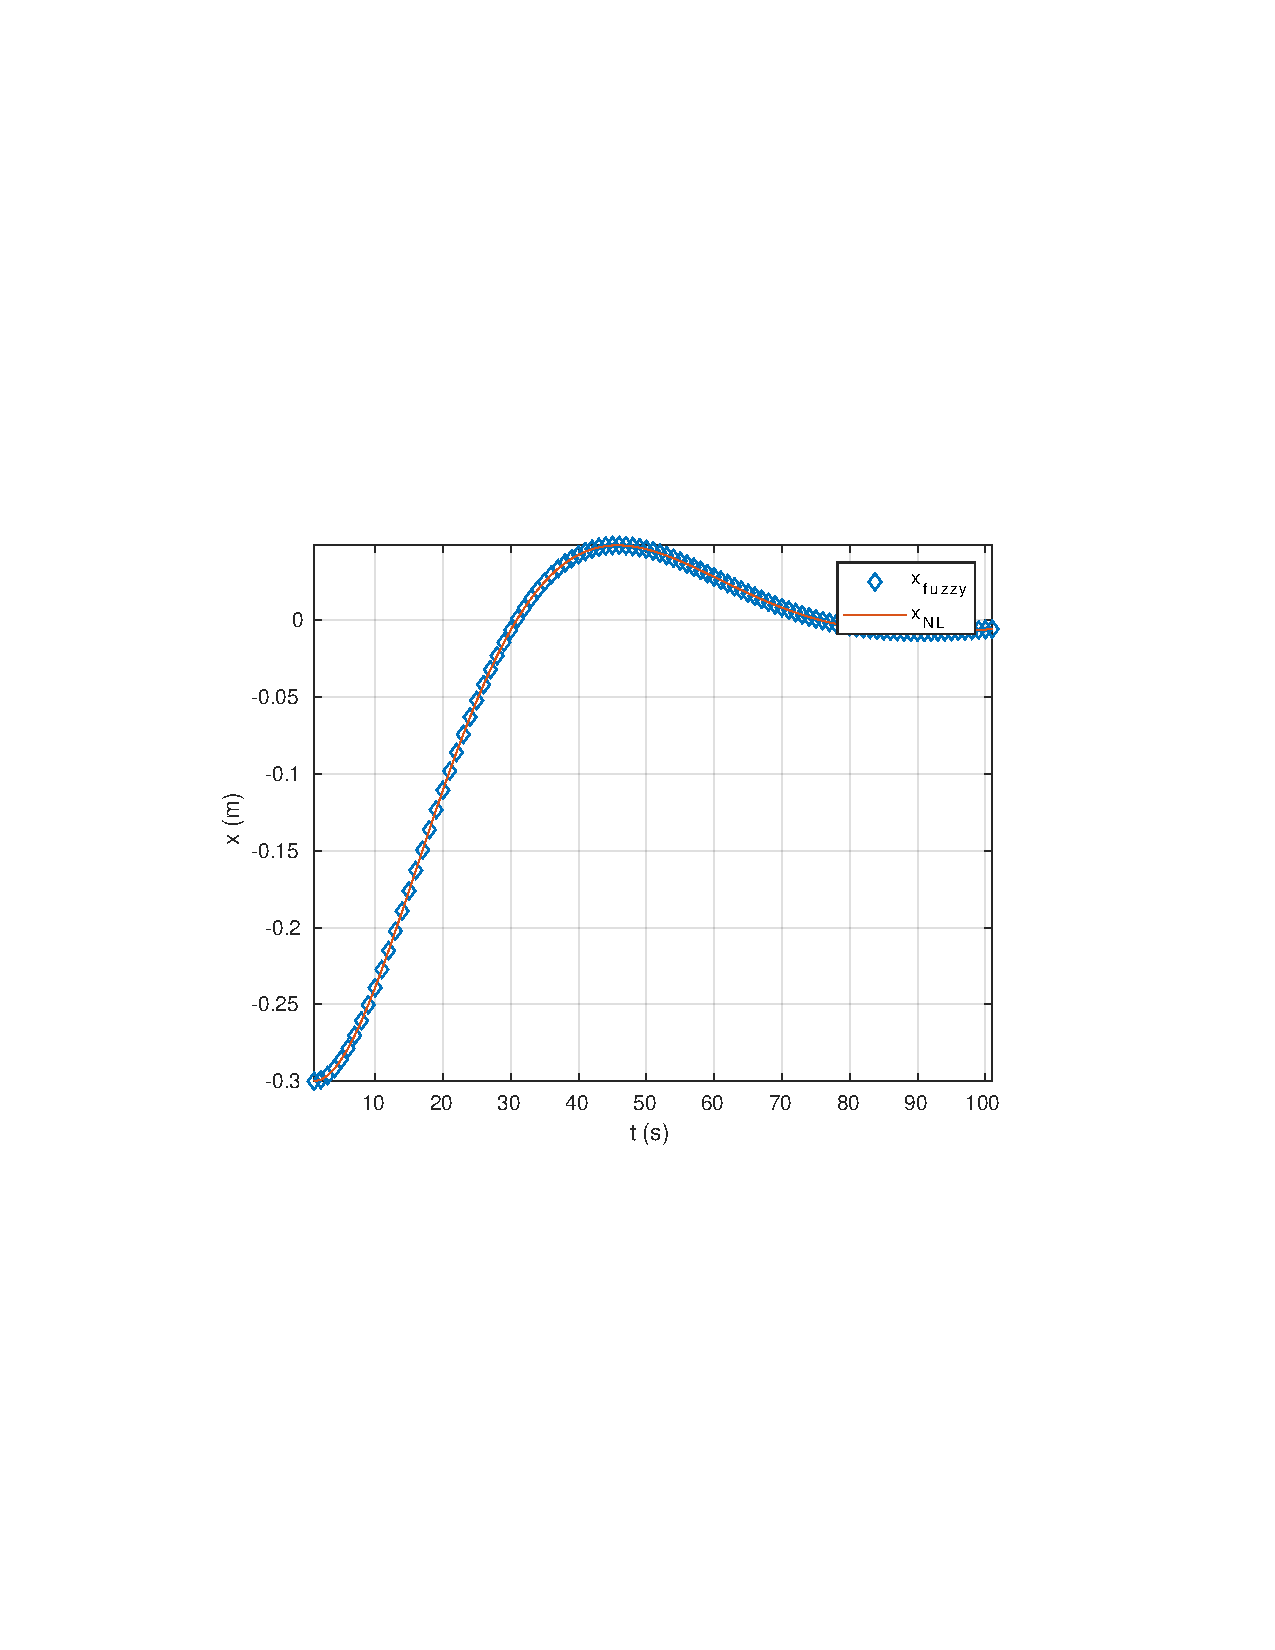
\includegraphics[scale=0.7,trim={3.5cm 8cm 4cm 8cm},clip]{figuras/OL/x.pdf} 
	\caption{Response of error system and its fuzzy approximation: $x$ coordinate} \label{fig:OL_x}
\end{figure} 
\end{frame}

\begin{frame}
	\begin{figure}[!htb]
		% \includegraphics[trim={5cm 0 0 0},clip]{example-image-a}
		% 	 trim={<left> <lower> <right> <upper>}
		\centering
		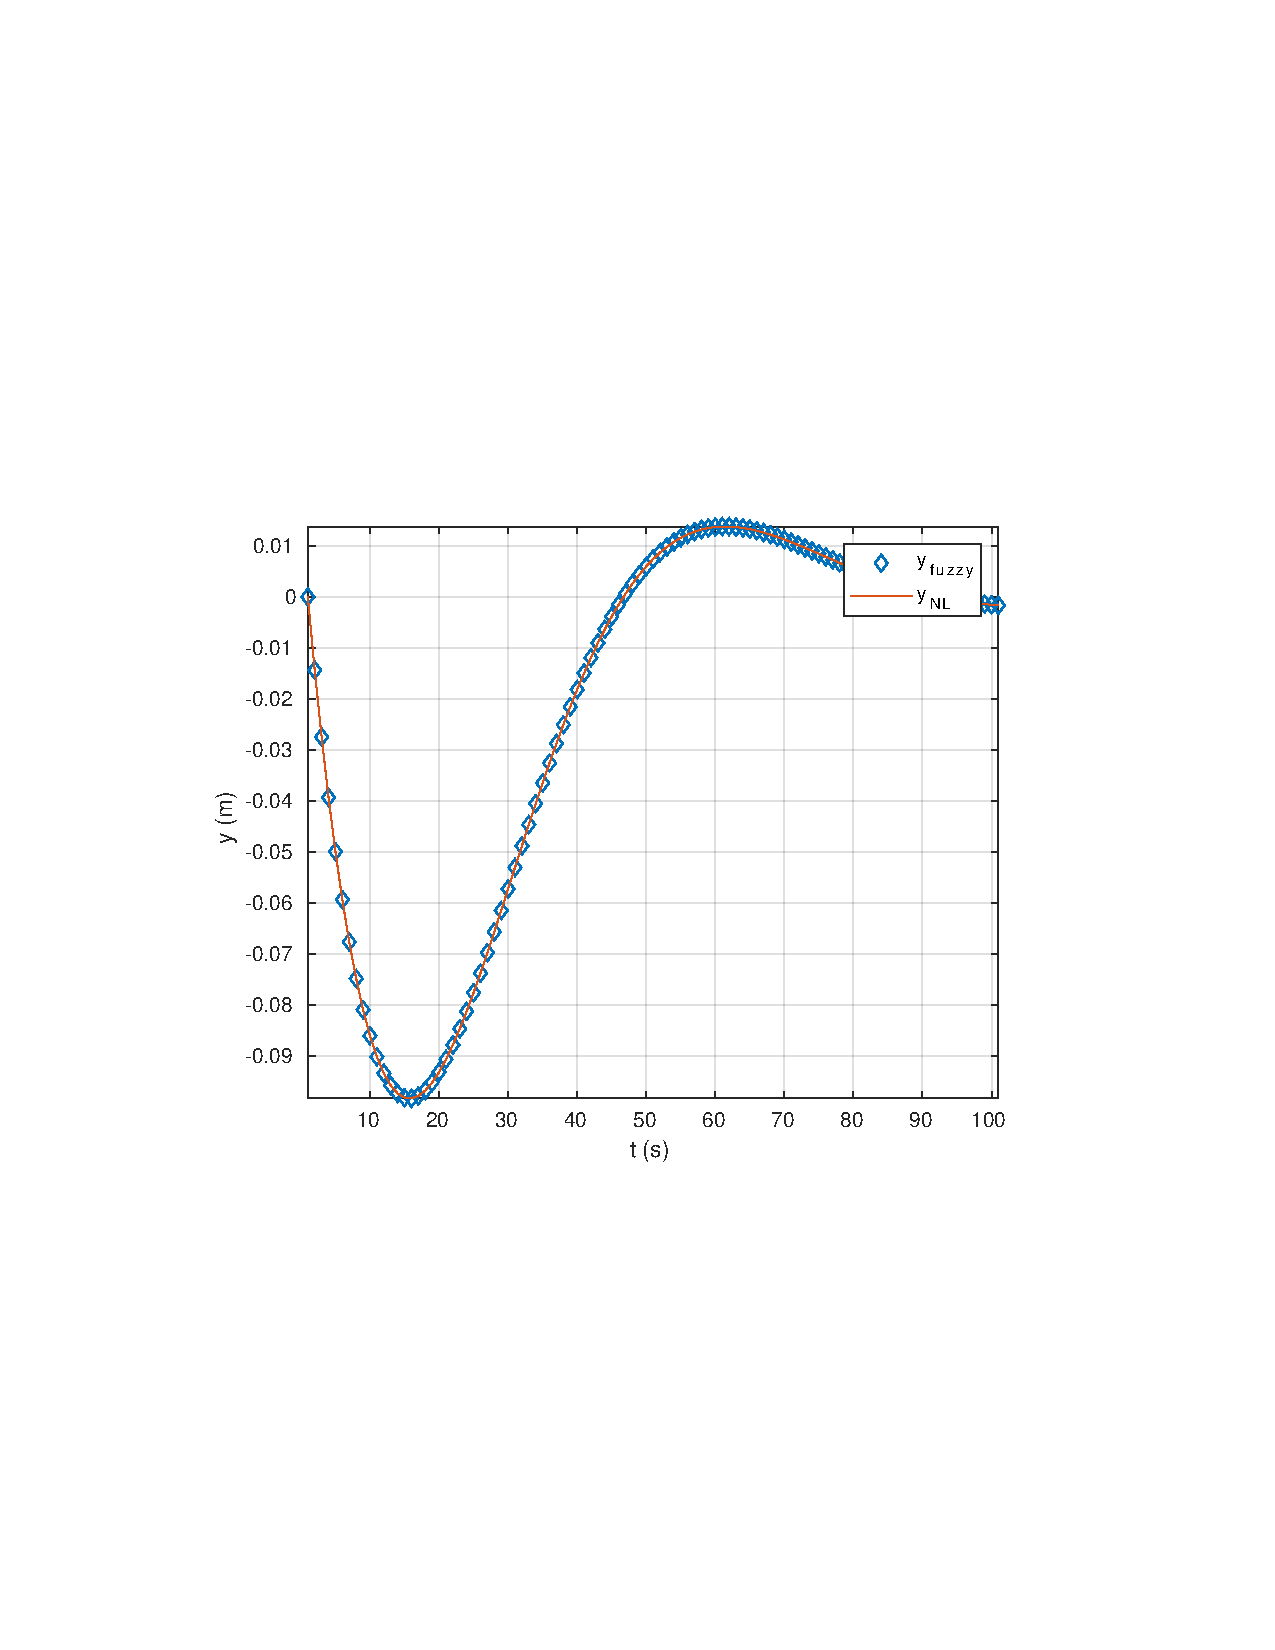
\includegraphics[scale=0.7,trim={3.5cm 8cm 4cm 8cm},clip]{figuras/OL/y.pdf}
		\caption{Response of error system and its fuzzy approximation: $y$ coordinate} \label{fig:OL_y}
	\end{figure} 
\end{frame}
%%%%%%%%%%%%%%%%%%%%%%%%%%%%%%%% FRAME %%%%%%%%%%%%%%%%%%%%%%%%%%%%%%%%
\begin{frame}
	\begin{figure}[!htb]
		% \includegraphics[trim={5cm 0 0 0},clip]{example-image-a}
		% 	 trim={<left> <lower> <right> <upper>}
		\centering
		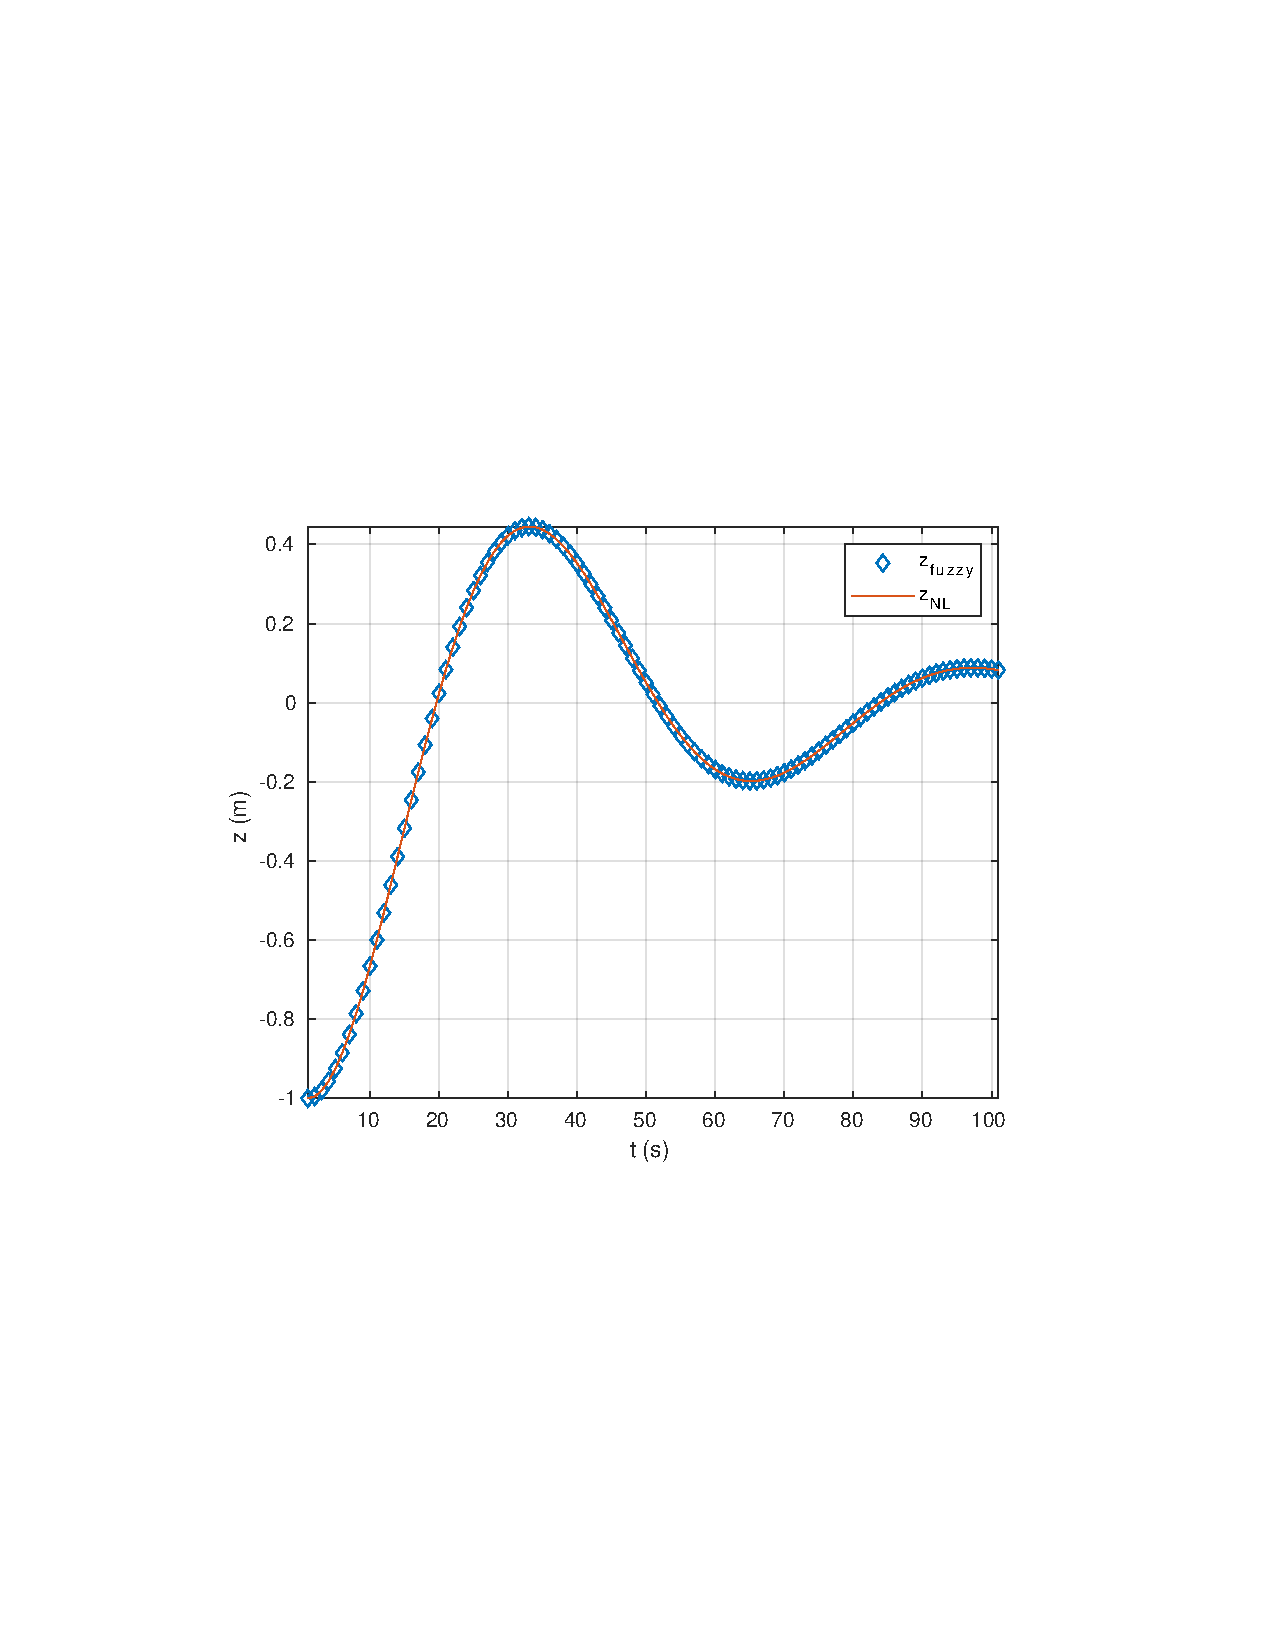
\includegraphics[scale=.7,trim={3.5cm 8cm 4cm 8cm},clip]{figuras/OL/z.pdf}
		\caption{Response of error system and its fuzzy approximation: $z$ coordinate} \label{fig:OL_z}
	\end{figure} 
\end{frame}

\begin{frame}
		\begin{figure}[!htb]
			% \includegraphics[trim={5cm 0 0 0},clip]{example-image-a}
			% 	 trim={<left> <lower> <right> <upper>}
			\centering
			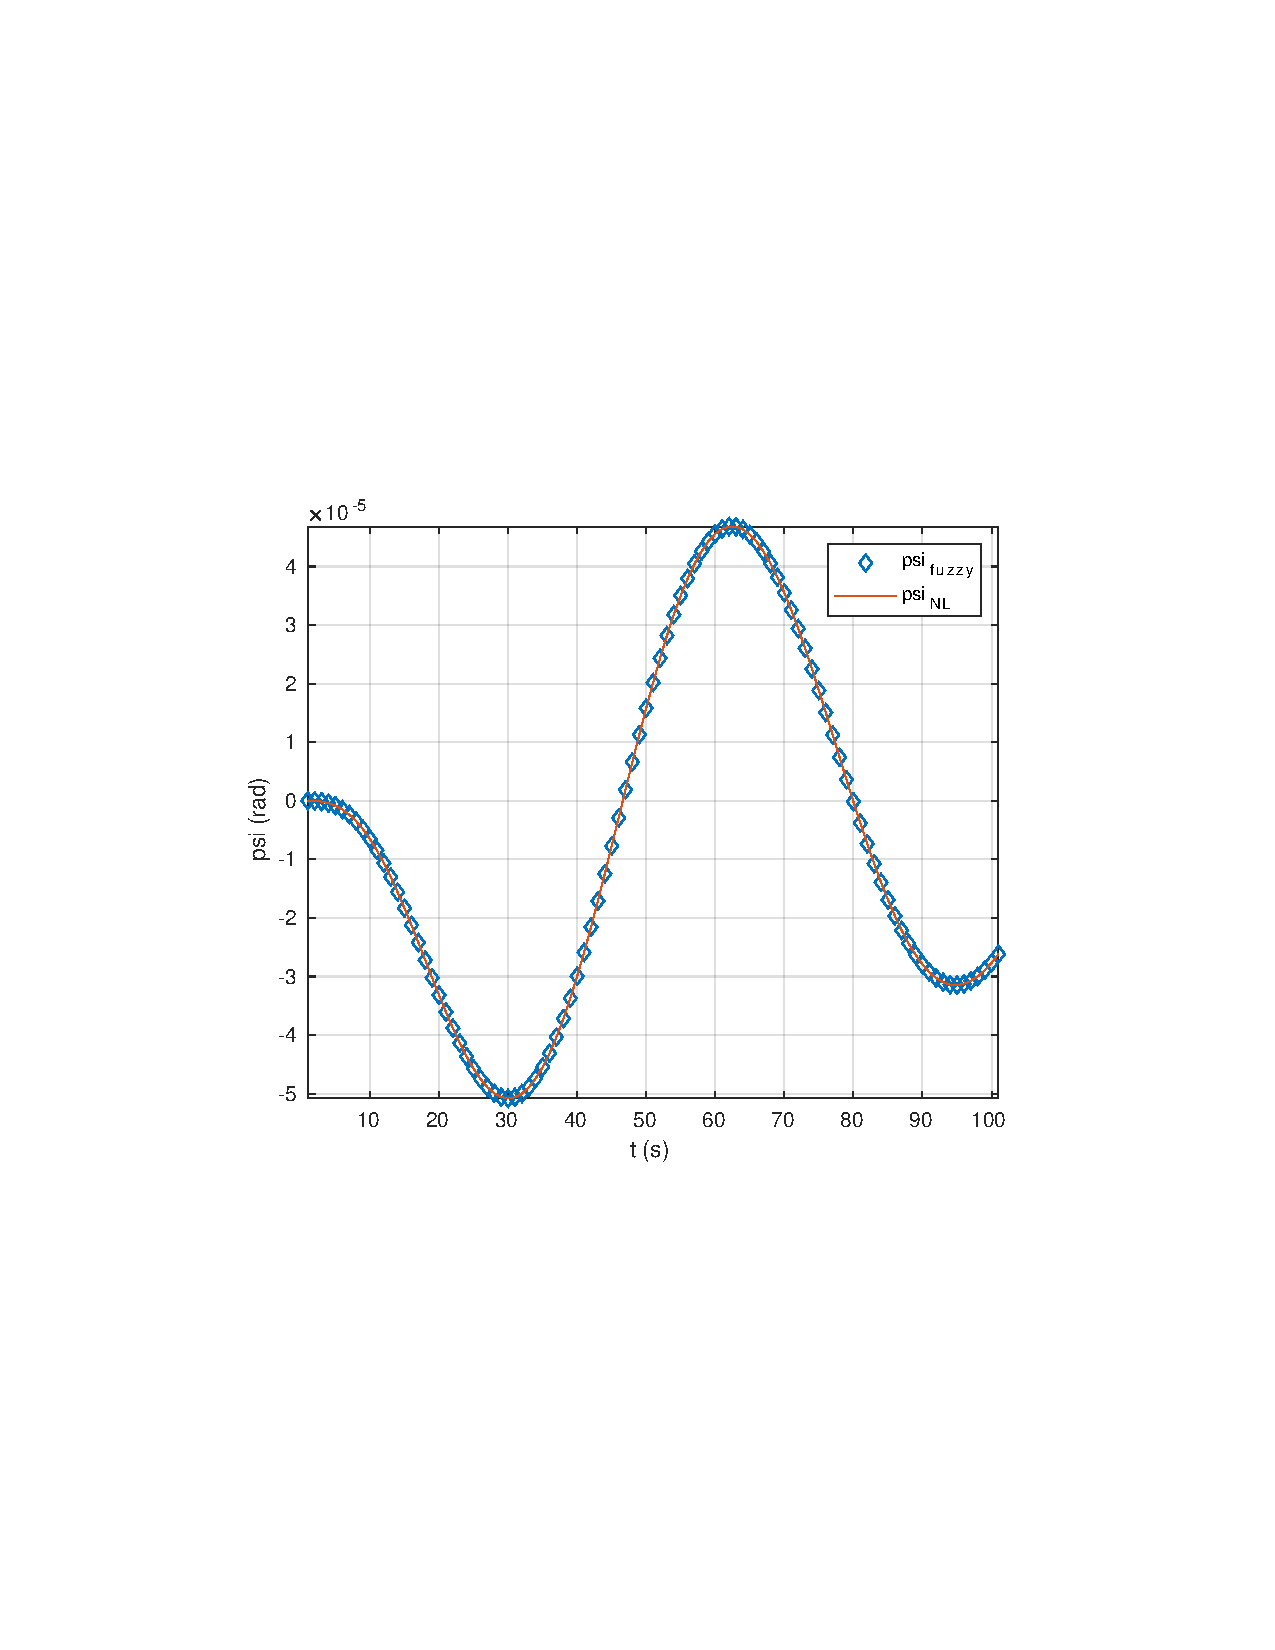
\includegraphics[scale=.7,trim={3.5cm 8cm 4cm 8cm},clip]{figuras/OL/psi.pdf}
			\caption{Response of error system and its fuzzy approximation: $\psi$ coordinate}
			\label{fig:OL_psi}
		\end{figure}
\end{frame}

%%%%%%%%%%%%%%%%%%%%%%%%%%%%%%%% FRAME %%%%%%%%%%%%%%%%%%%%%%%%%%%%%%%%

\begin{frame}{Indoor Experiments}
 \begin{table}[!htb]
 	\centering
 	\caption{Indoor Experiments}
 	\begin{tabular}{||c c c c||} 
 		\hline
 		Trajectory & $a$ (m) & $v$ (m/s) & Position Sensor  \\ %[0.5ex] 
 		\hline\hline
 		Circle & $0.3$ & $0.1$ & Vicon \\
 		Gerono Lemniscate & $0.4$ & $0.1$ & Vicon \\
 		\hline
 	\end{tabular}
 	\label{table:indoor}
 \end{table}
\end{frame}

%%%%%%%%%%%%%%%%%%%%%%%%%%%%%%%% FRAME %%%%%%%%%%%%%%%%%%%%%%%%%%%%%%%%

\begin{frame}
\begin{figure}[!htb]
	% \includegraphics[trim={5cm 0 0 0},clip]{example-image-a}
	% 	 trim={<left> <lower> <right> <upper>}
	\centering
	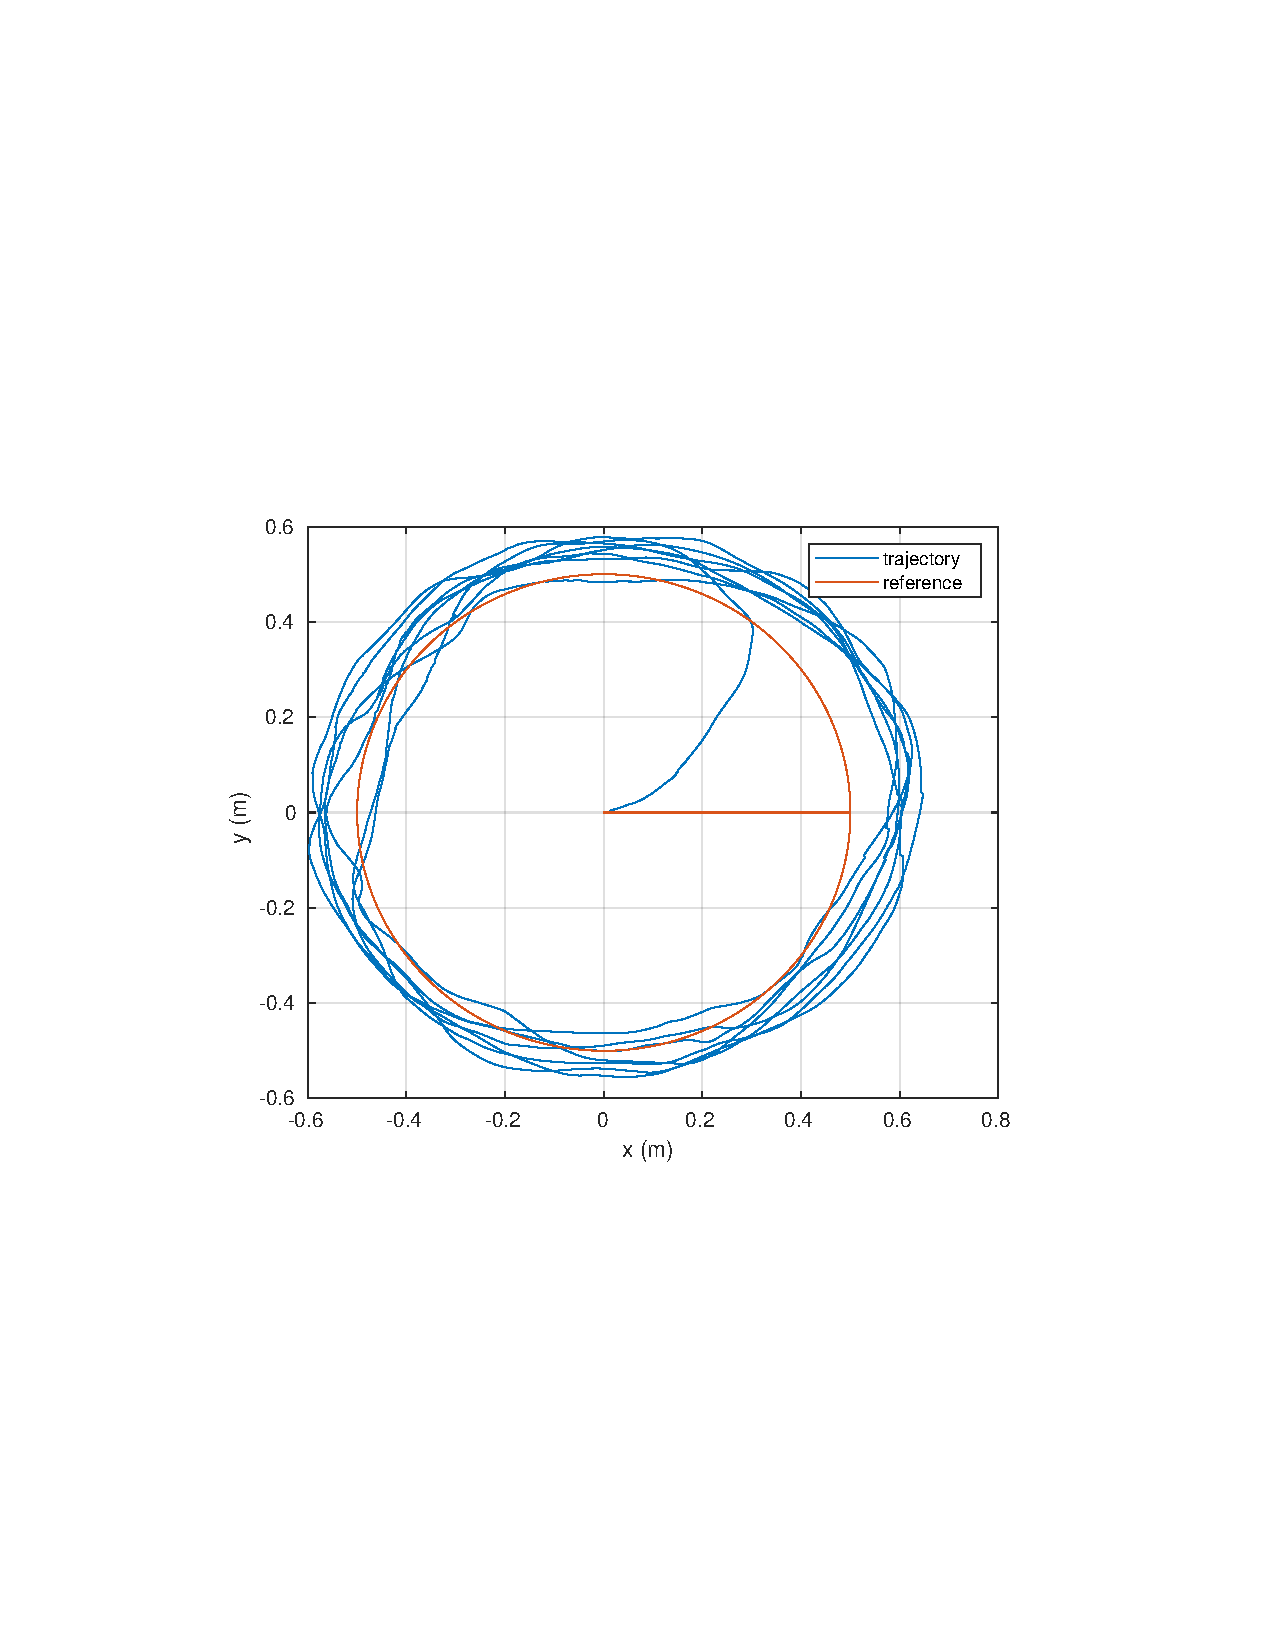
\includegraphics[scale=.7,trim={3.5cm 8cm 4cm 8cm},clip]{figuras/CROB_Fuzzy_vel01_a05_circleXY/circle.pdf}
	\caption{The circle trajectory}
	\label{fig:crob_circ}
\end{figure}
\end{frame}
%%%%%%%%%%%%%%%%%%%%%%%%%%%%%%%% FRAME %%%%%%%%%%%%%%%%%%%%%%%%%%%%%%%%
\begin{frame}
	\begin{figure}[!htb]
		% \includegraphics[trim={5cm 0 0 0},clip]{example-image-a}
		% 	 trim={<left> <lower> <right> <upper>}
		\centering
		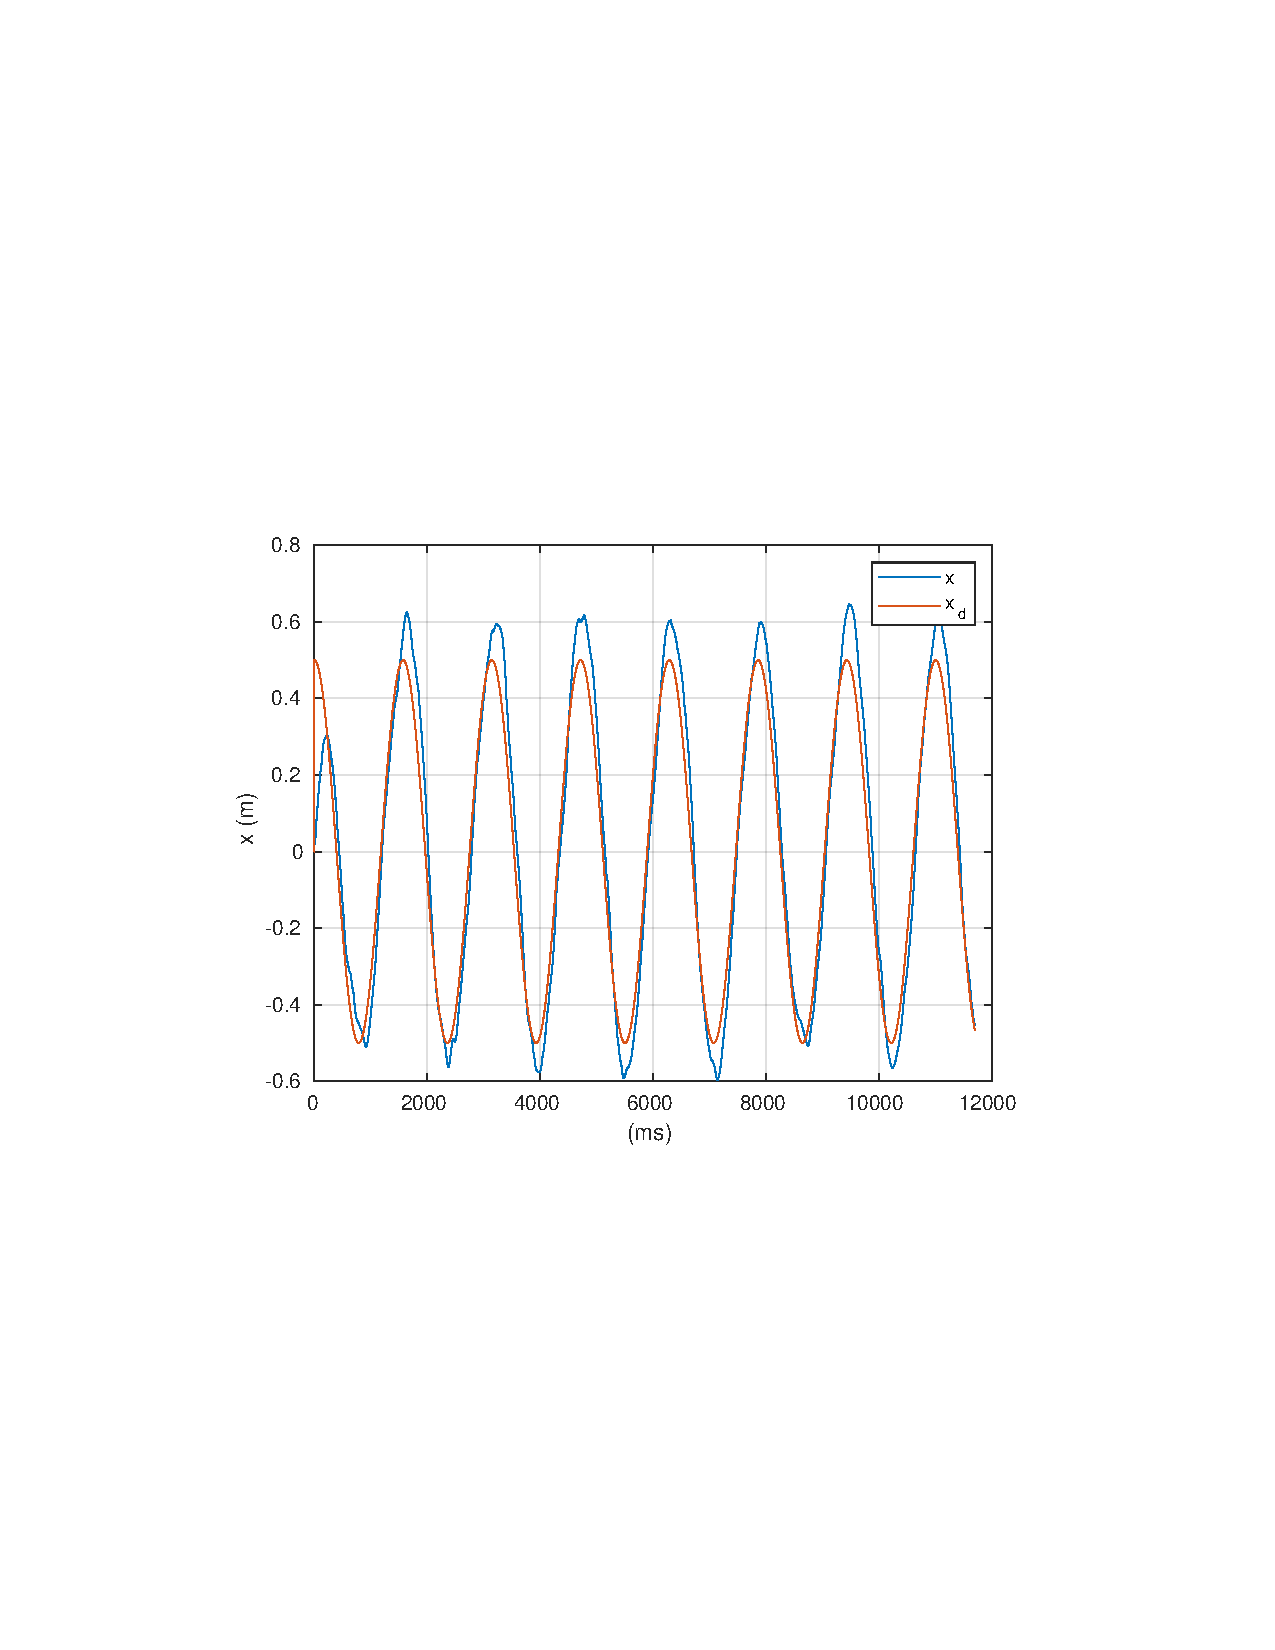
\includegraphics[scale=.7,trim={3.5cm 8cm 4cm 8cm},clip]{figuras/CROB_Fuzzy_vel01_a05_circleXY/x.pdf}
		\caption{$x(t)$ for the circle}
		\label{fig:crob_circ_x}
	\end{figure}
\end{frame}
%%%%%%%%%%%%%%%%%%%%%%%%%%%%%%%% FRAME %%%%%%%%%%%%%%%%%%%%%%%%%%%%%%%%
\begin{frame}
		\begin{figure}[!htb]
			% \includegraphics[trim={5cm 0 0 0},clip]{example-image-a}
			% 	 trim={<left> <lower> <right> <upper>}
			\centering
			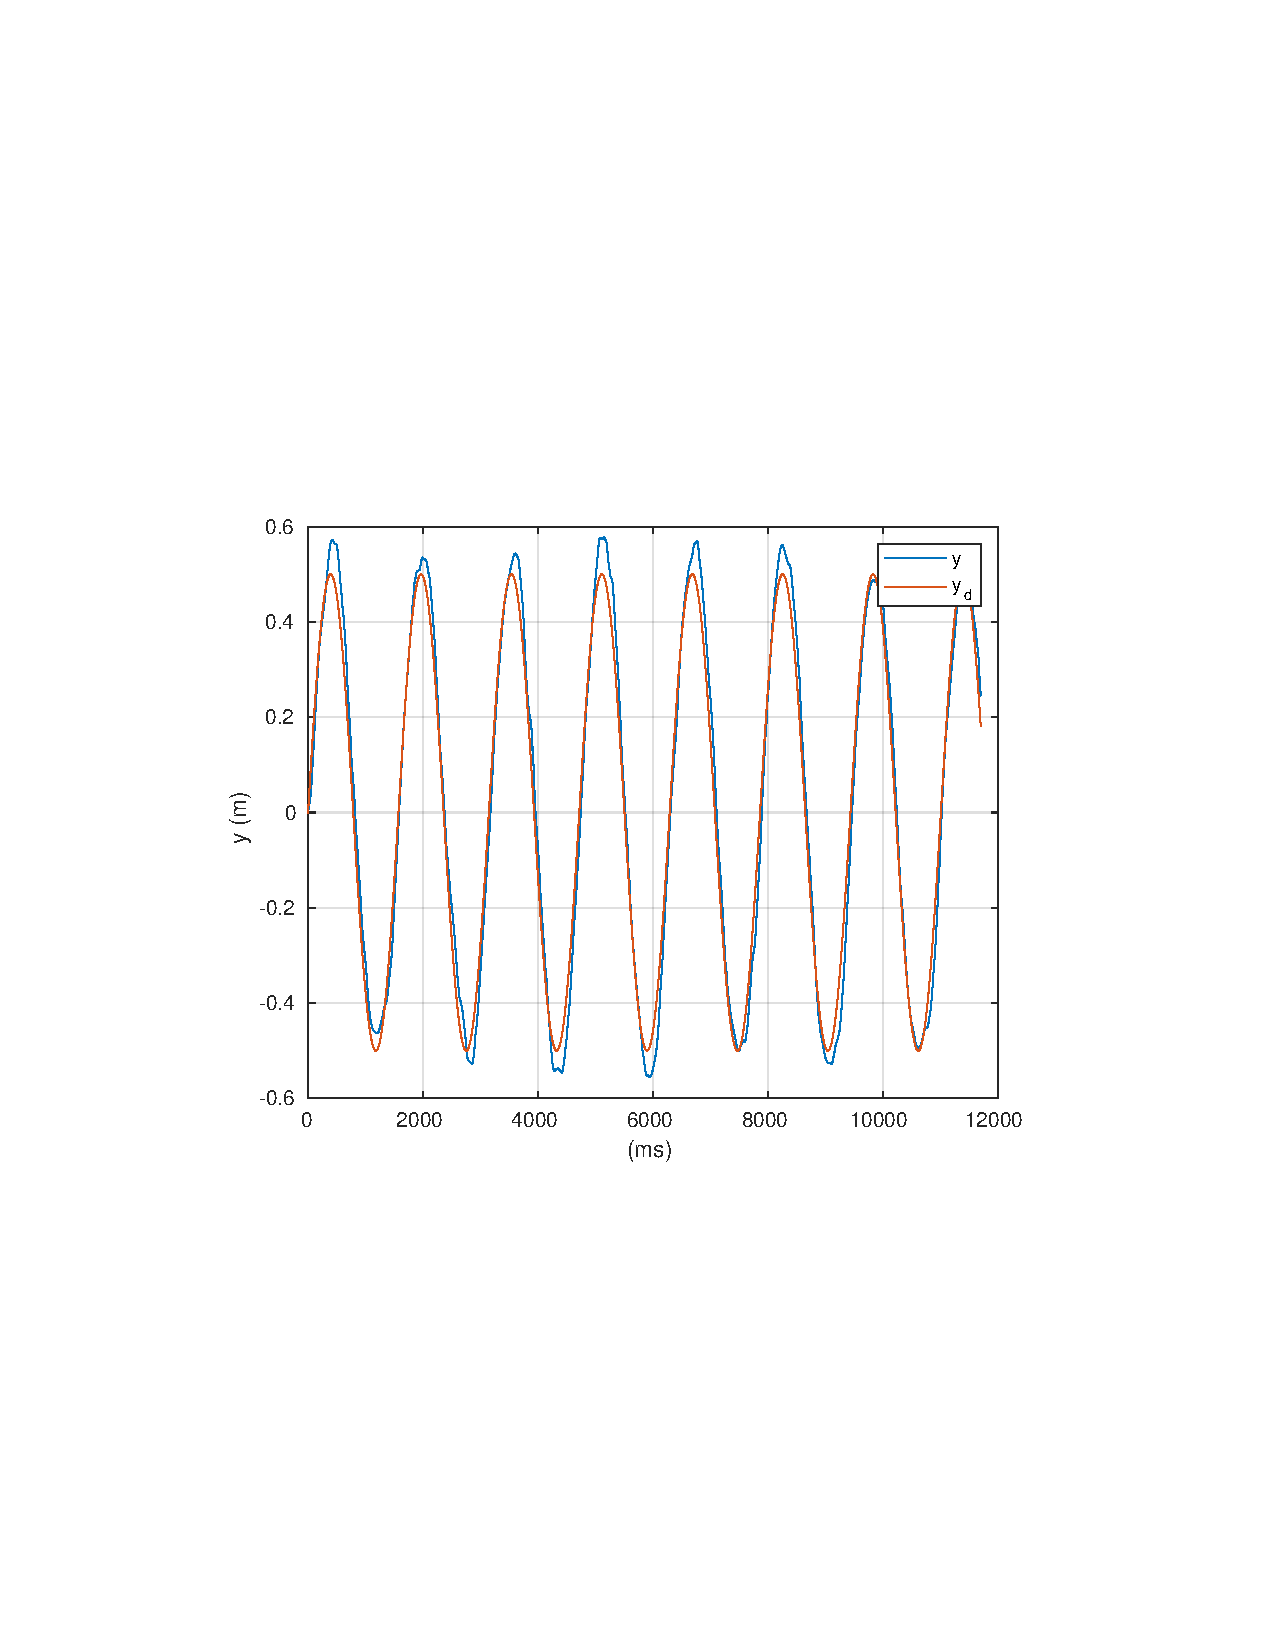
\includegraphics[scale=0.7,trim={3.5cm 8cm 4cm 8cm},clip]{figuras/CROB_Fuzzy_vel01_a05_circleXY/y.pdf}
			\caption{$y(t)$ for the circle}
			\label{fig:crob_circ_y}
		\end{figure}
\end{frame}
%%%%%%%%%%%%%%%%%%%%%%%%%%%%%%%% FRAME %%%%%%%%%%%%%%%%%%%%%%%%%%%%%%%%
\begin{frame}
	\begin{figure}[!htb]
		% \includegraphics[trim={5cm 0 0 0},clip]{example-image-a}
		% 	 trim={<left> <lower> <right> <upper>}
		\centering
		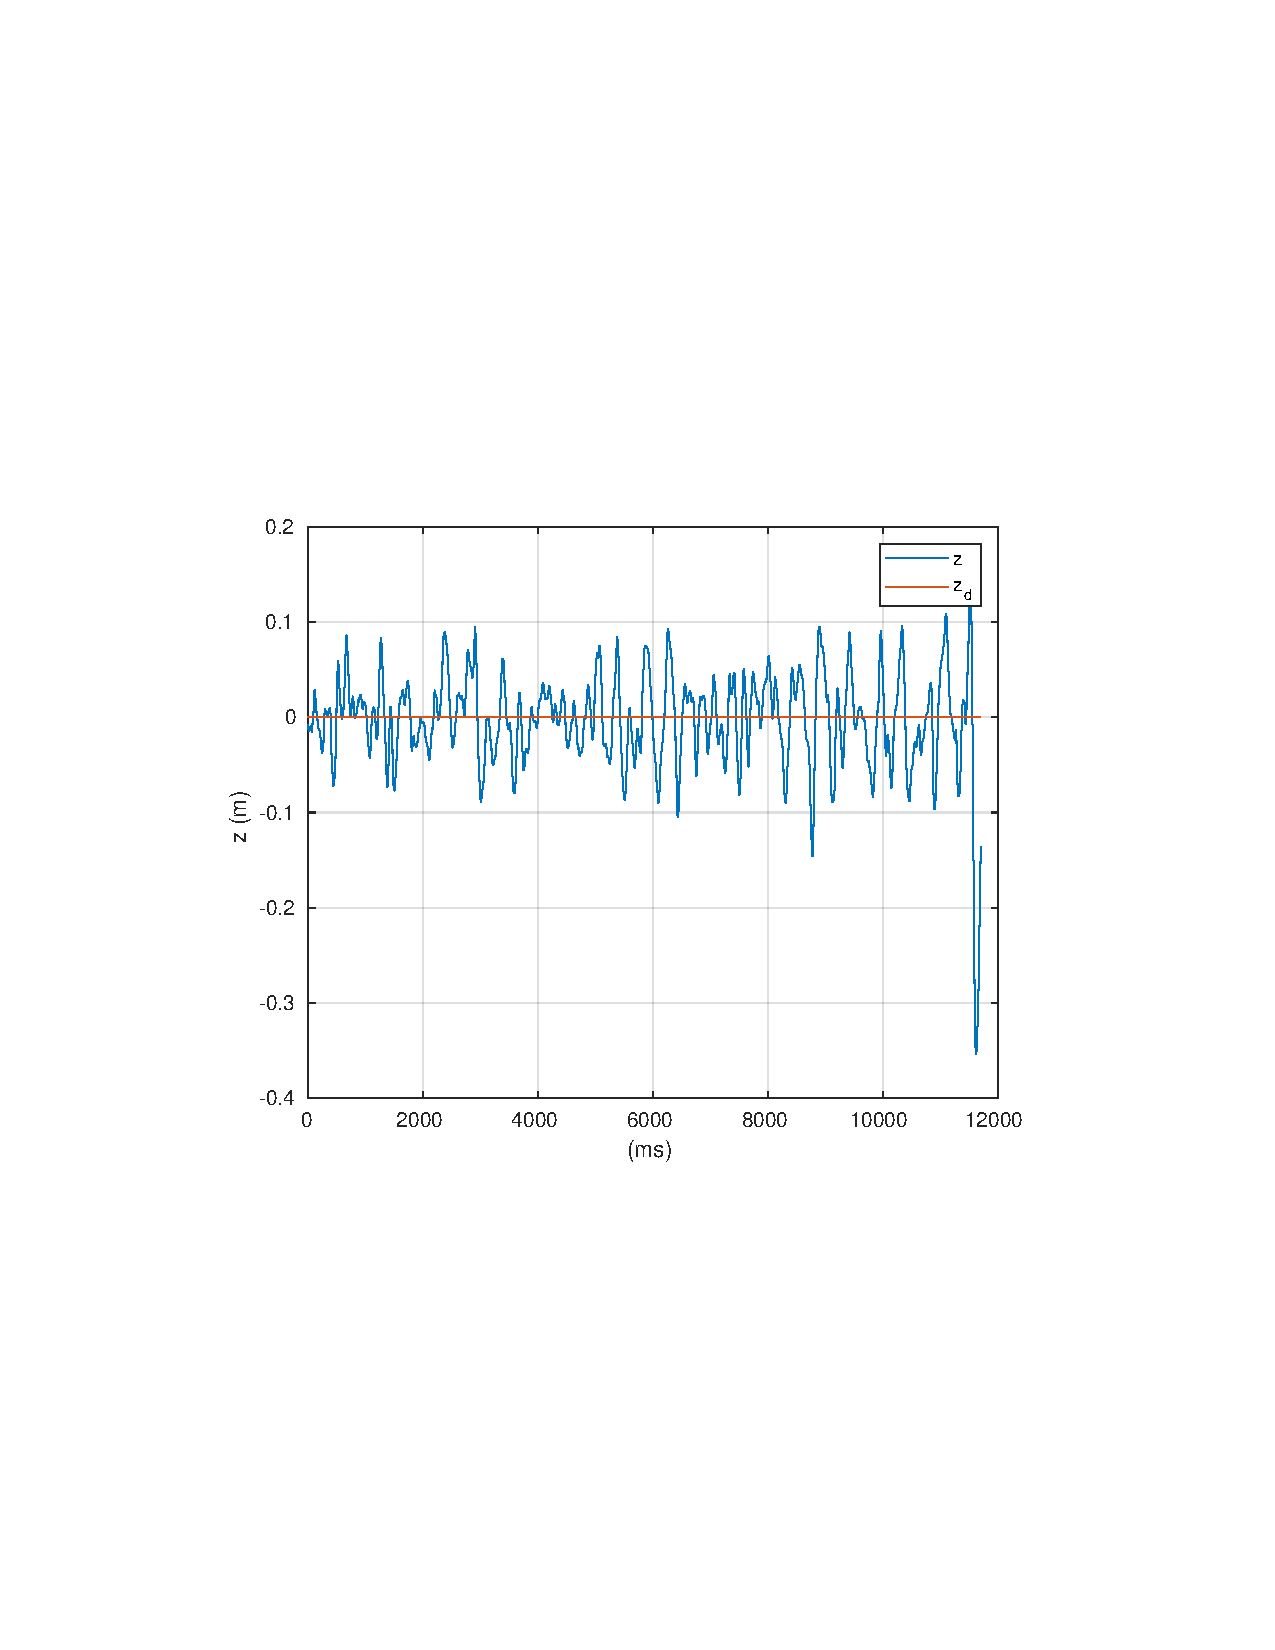
\includegraphics[scale=.7,trim={3.5cm 8cm 4cm 8cm},clip]{figuras/CROB_Fuzzy_vel01_a05_circleXY/z.pdf}
		\caption{$z(t)$ for the circle}
		\label{fig:crob_circ_z}
	\end{figure}
\end{frame}
%%%%%%%%%%%%%%%%%%%%%%%%%%%%%%%% FRAME %%%%%%%%%%%%%%%%%%%%%%%%%%%%%%%%
\begin{frame}
		\begin{figure}[!htb]
			% \includegraphics[trim={5cm 0 0 0},clip]{example-image-a}
			% 	 trim={<left> <lower> <right> <upper>}
			\centering
			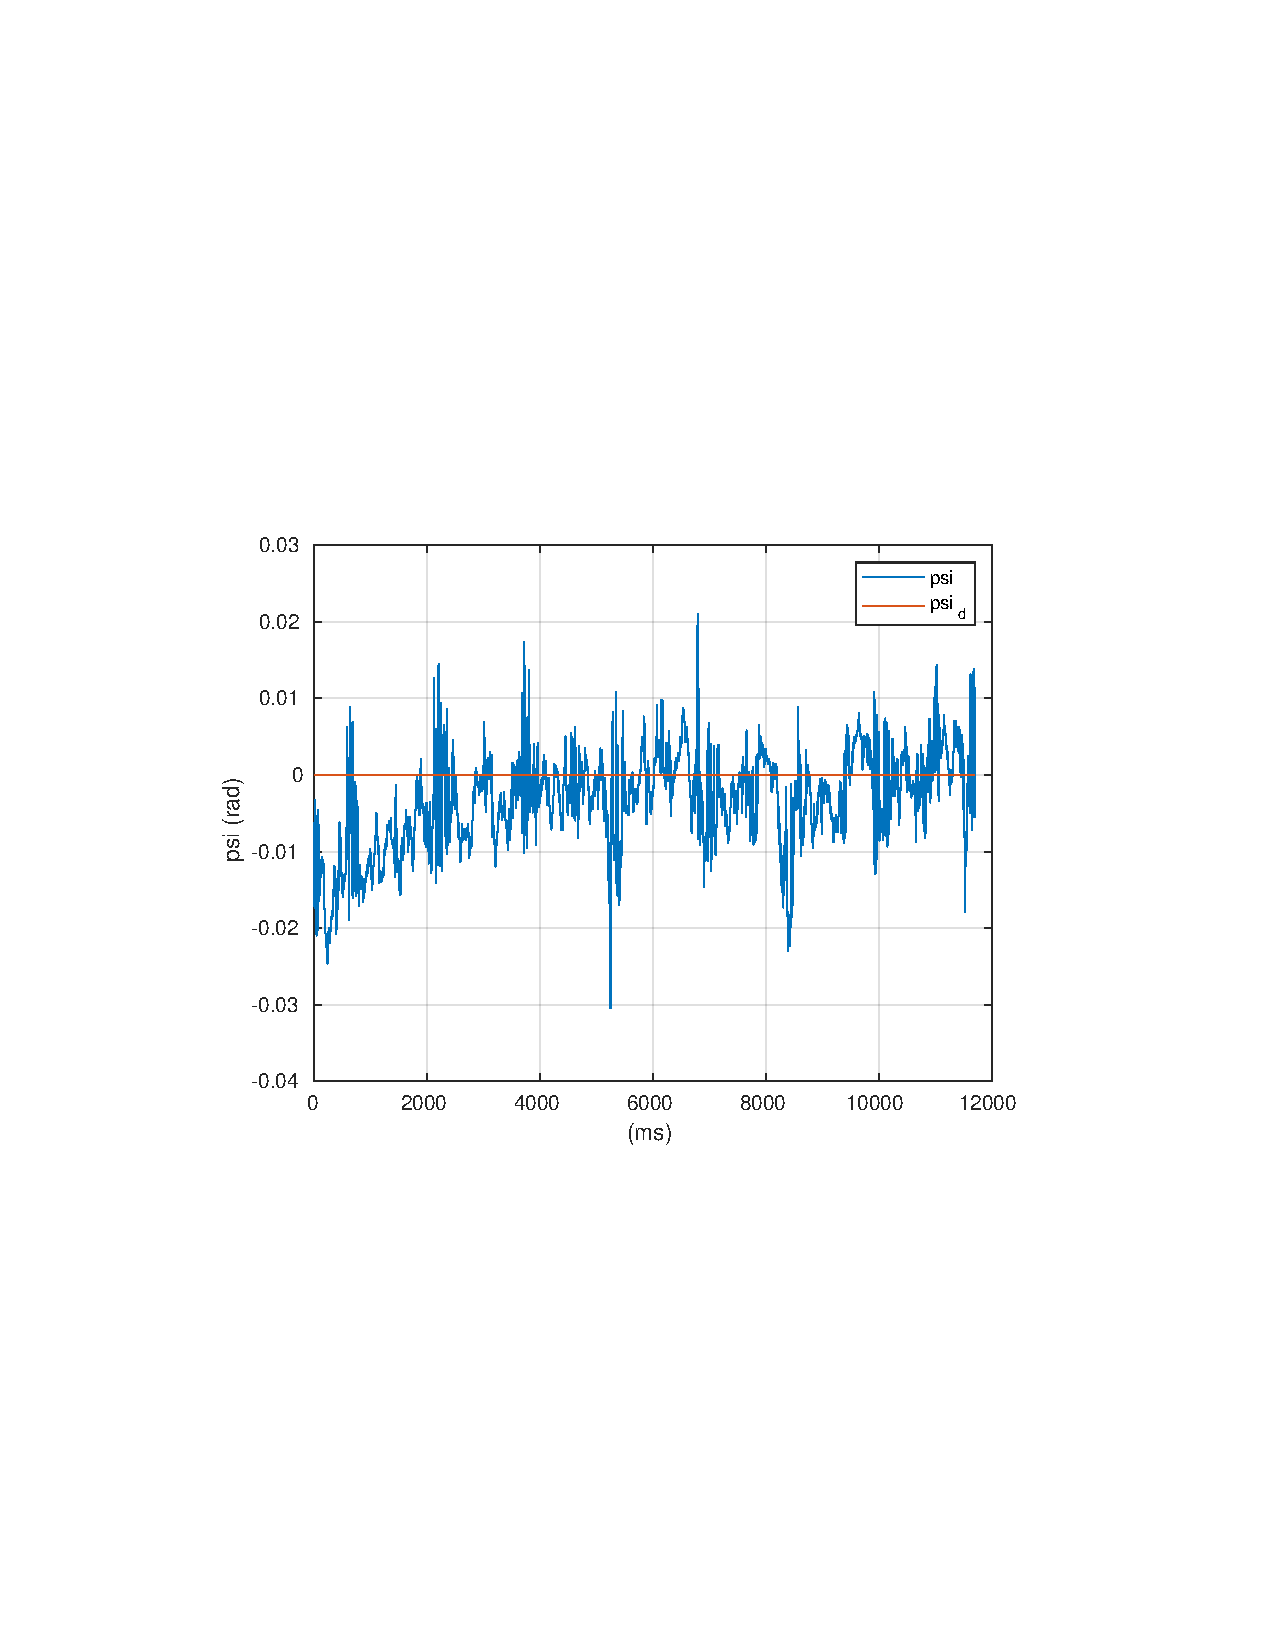
\includegraphics[scale=.7,trim={3.5cm 8cm 4cm 8cm},clip]{figuras/CROB_Fuzzy_vel01_a05_circleXY/psi.pdf}
			\caption{$\psi(t)$ for the circle}
			\label{fig:crob_circ_psi}
		\end{figure}
\end{frame}
%%%%%%%%%%%%%%%%%%%%%%%%%%%%%%%% FRAME %%%%%%%%%%%%%%%%%%%%%%%%%%%%%%%%
\begin{frame}
 \begin{figure}[!htb]
 	% \includegraphics[trim={5cm 0 0 0},clip]{example-image-a}
 	% 	 trim={<left> <lower> <right> <upper>}
 	\centering
 	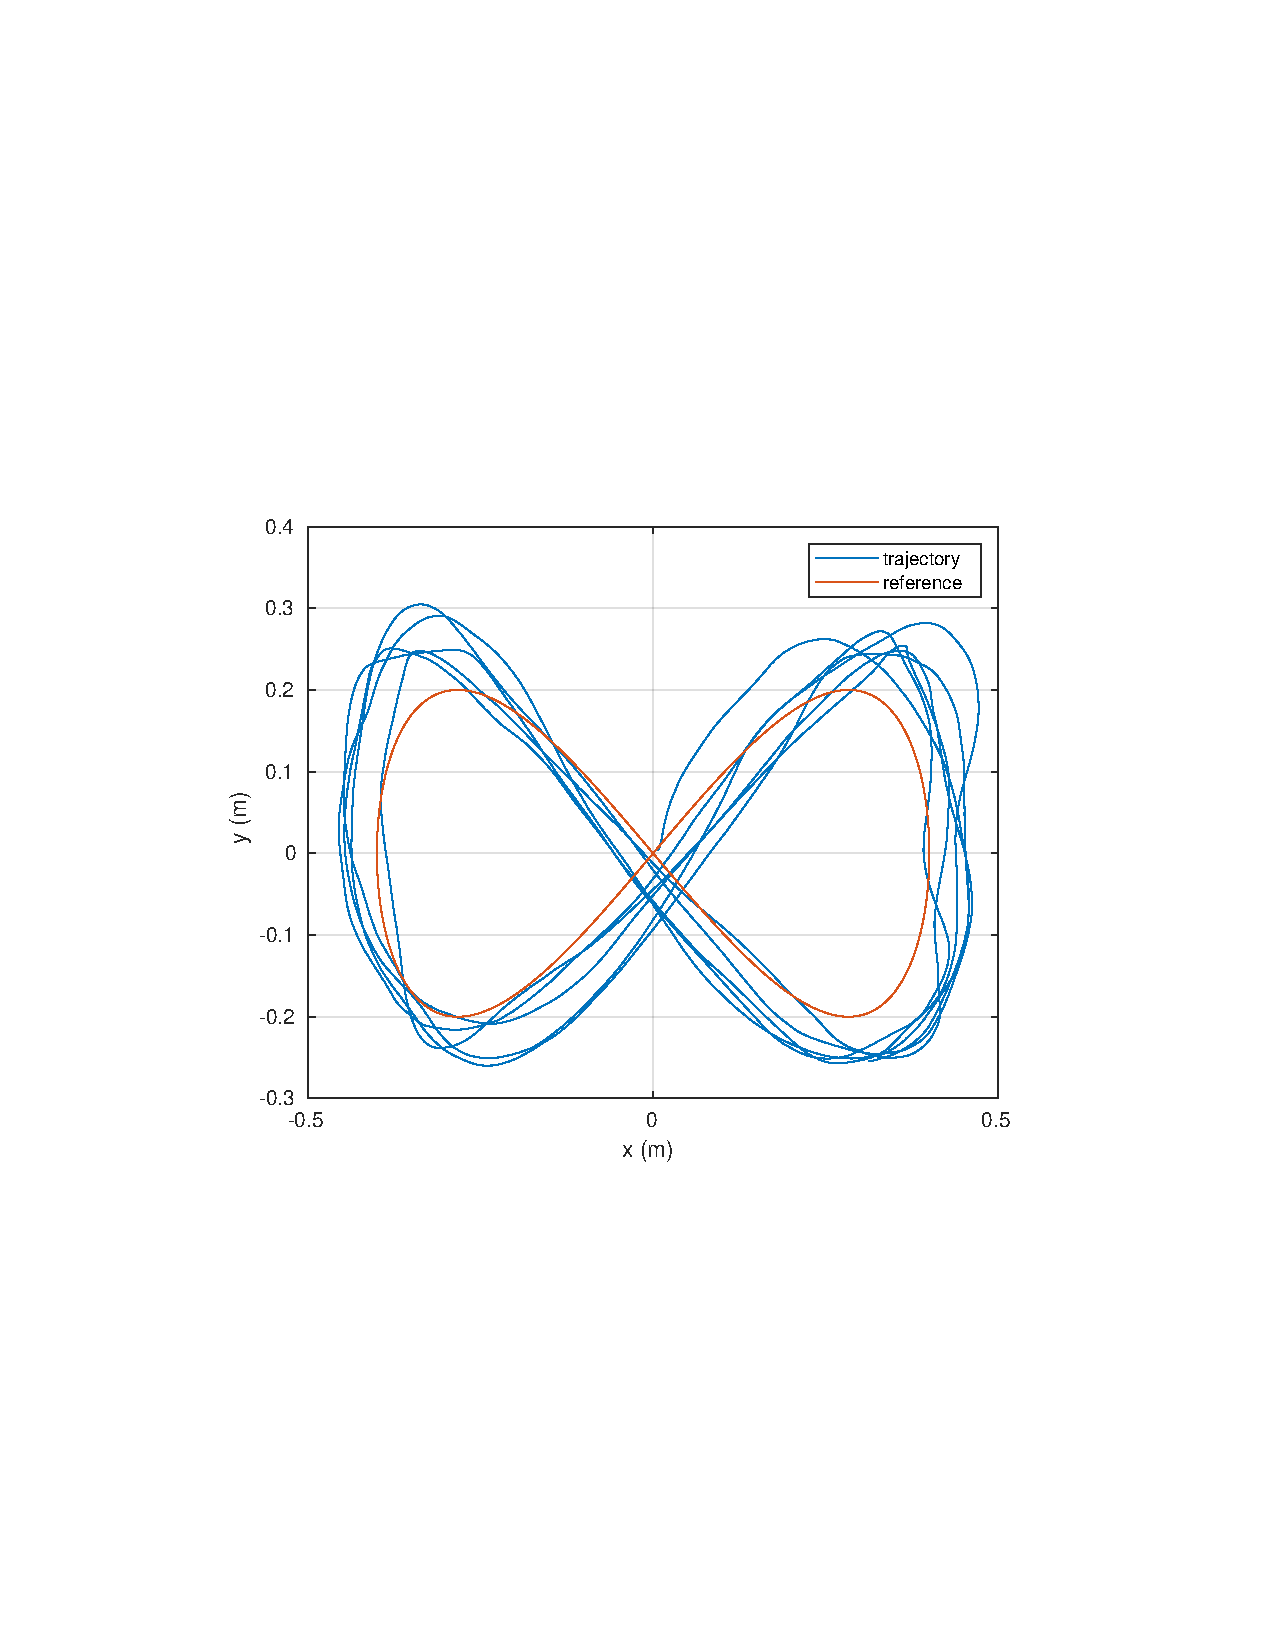
\includegraphics[scale=.7,trim={3.5cm 8cm 4cm 8cm},clip]{figuras/CROB_Fuzzy_Gerono/ref.pdf}
 	\caption{The Gerono Lemniscate trajectory}
 	\label{fig:crob_lem}
 \end{figure}
\end{frame}
%%%%%%%%%%%%%%%%%%%%%%%%%%%%%%%% FRAME %%%%%%%%%%%%%%%%%%%%%%%%%%%%%%%%
\begin{frame} 
 \begin{figure}[!htb]
 	% \includegraphics[trim={5cm 0 0 0},clip]{example-image-a}
 	% 	 trim={<left> <lower> <right> <upper>}
 	\centering
 	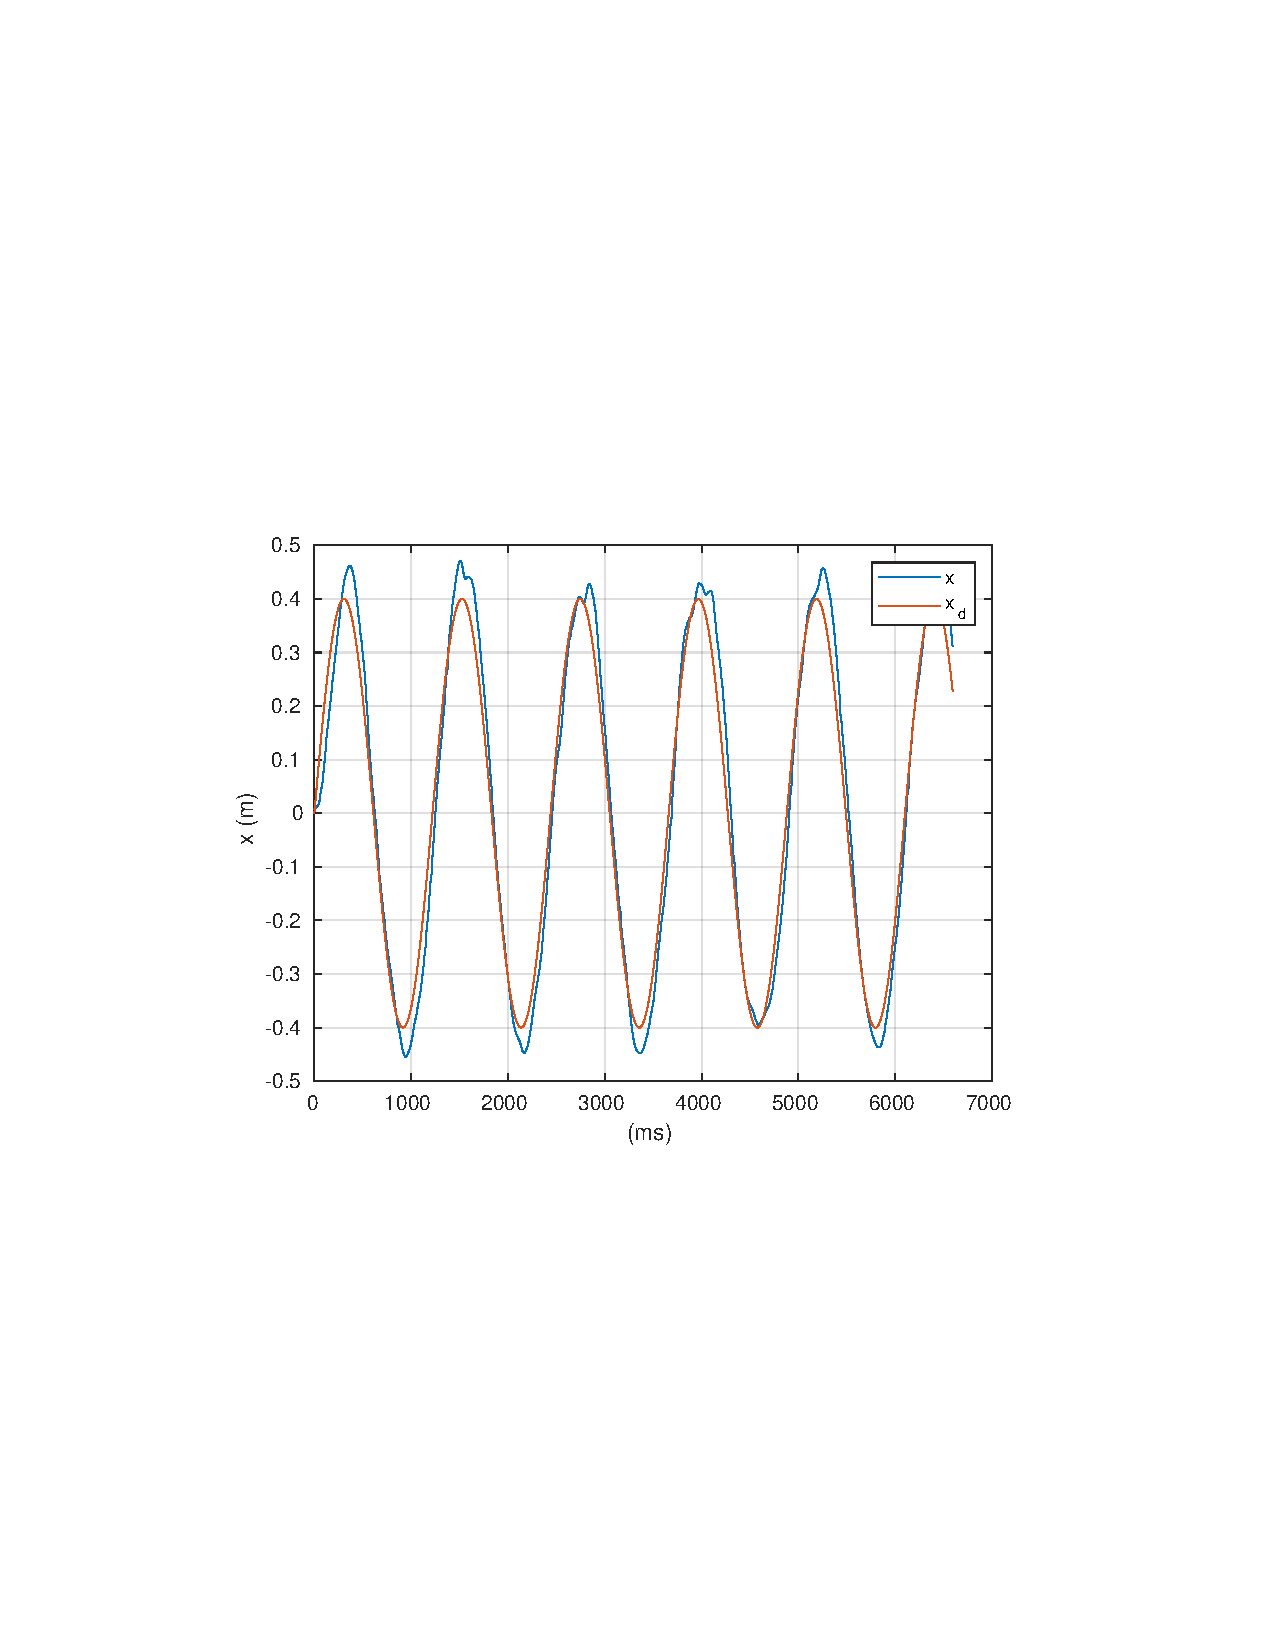
\includegraphics[scale=0.7,trim={3.5cm 8cm 4cm 8cm},clip]{figuras/CROB_Fuzzy_Gerono/x.pdf}
 	\caption{$x(t)$ for the Lemniscate of Gerono}
 	\label{fig:crob_lem_x}
 \end{figure}
\end{frame}
%%%%%%%%%%%%%%%%%%%%%%%%%%%%%%%% FRAME %%%%%%%%%%%%%%%%%%%%%%%%%%%%%%%%
\begin{frame} 
 \begin{figure}[!htb]
 	% \includegraphics[trim={5cm 0 0 0},clip]{example-image-a}
 	% 	 trim={<left> <lower> <right> <upper>}
 	\centering
 	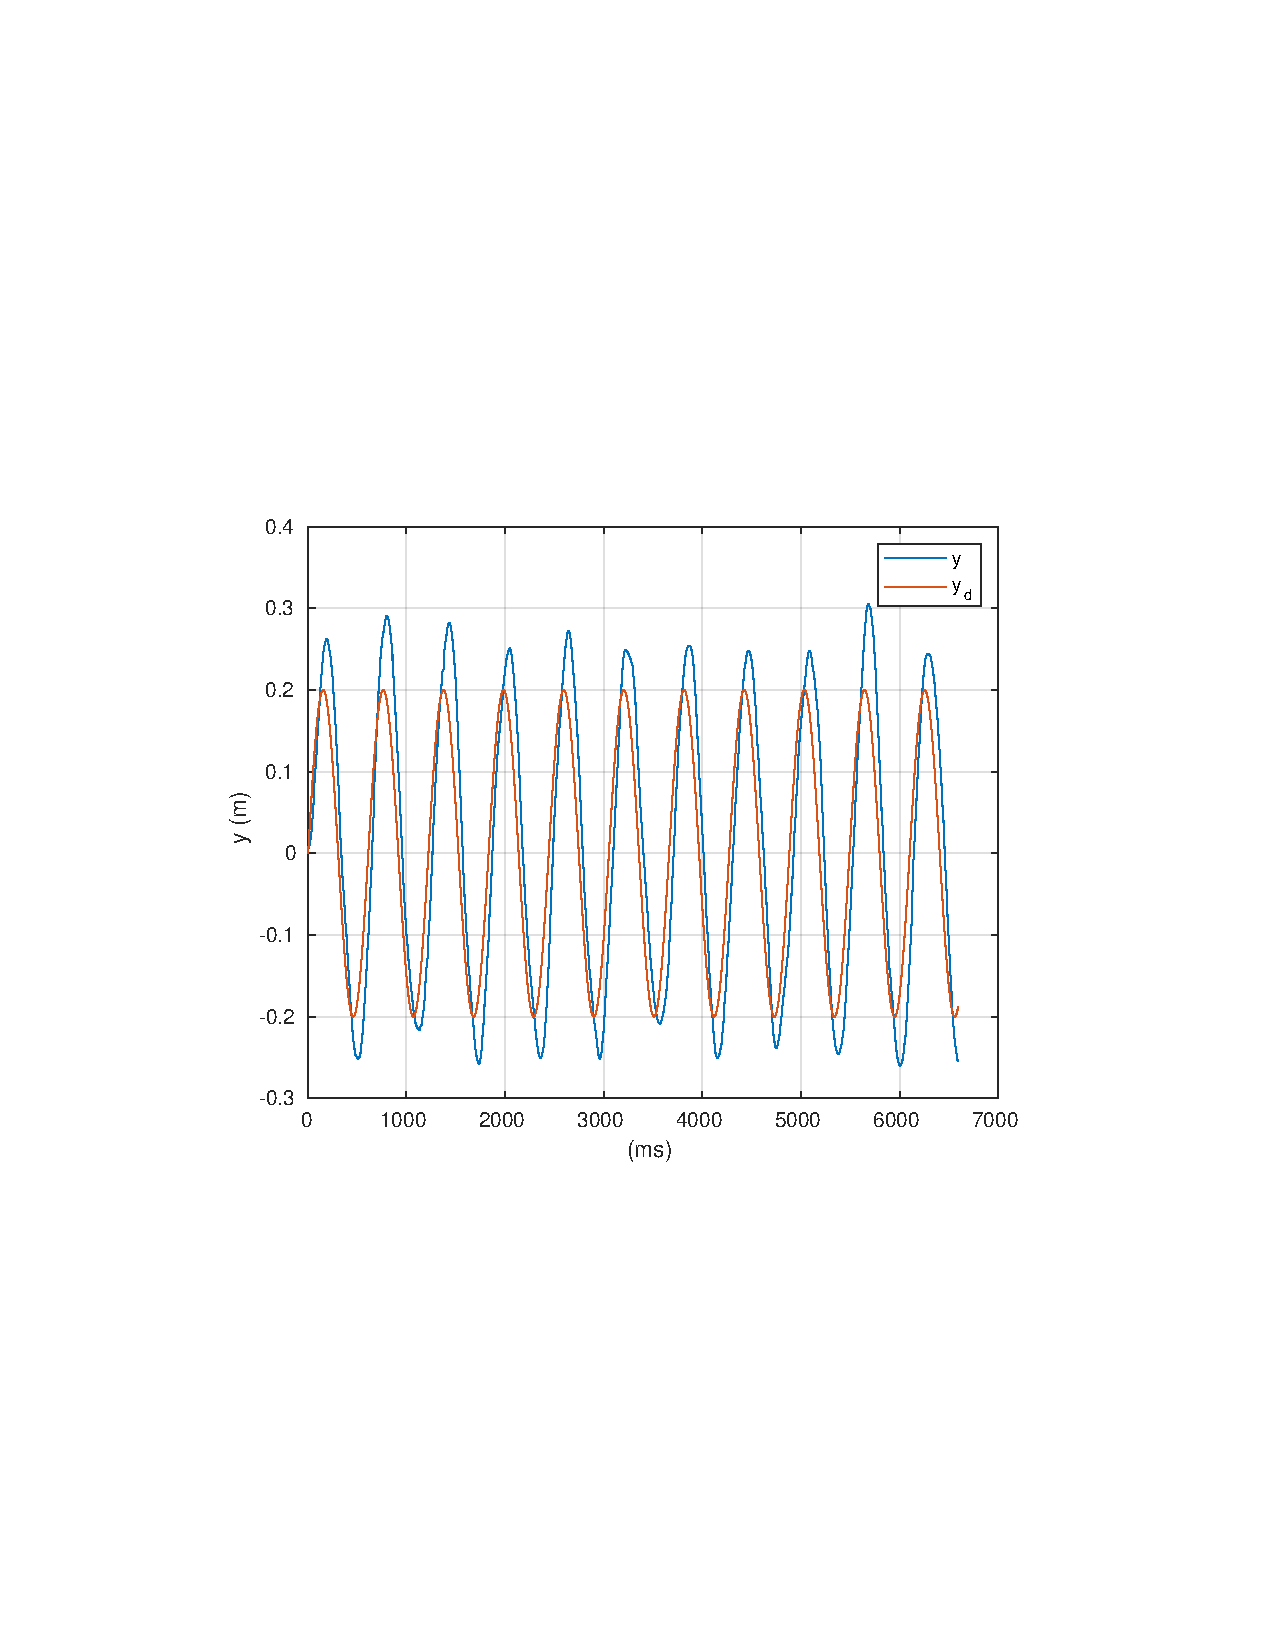
\includegraphics[scale=0.7,trim={3.5cm 8cm 4cm 8cm},clip]{figuras/CROB_Fuzzy_Gerono/y.pdf}
 	\caption{$y(t)$ for the Lemniscate of Gerono}
 	\label{fig:crob_lem_y}
 \end{figure} 
\end{frame}
%%%%%%%%%%%%%%%%%%%%%%%%%%%%%%%% FRAME %%%%%%%%%%%%%%%%%%%%%%%%%%%%%%%%
\begin{frame}
	\begin{figure}[!htb]
		% \includegraphics[trim={5cm 0 0 0},clip]{example-image-a}
		% 	 trim={<left> <lower> <right> <upper>}
		\centering
		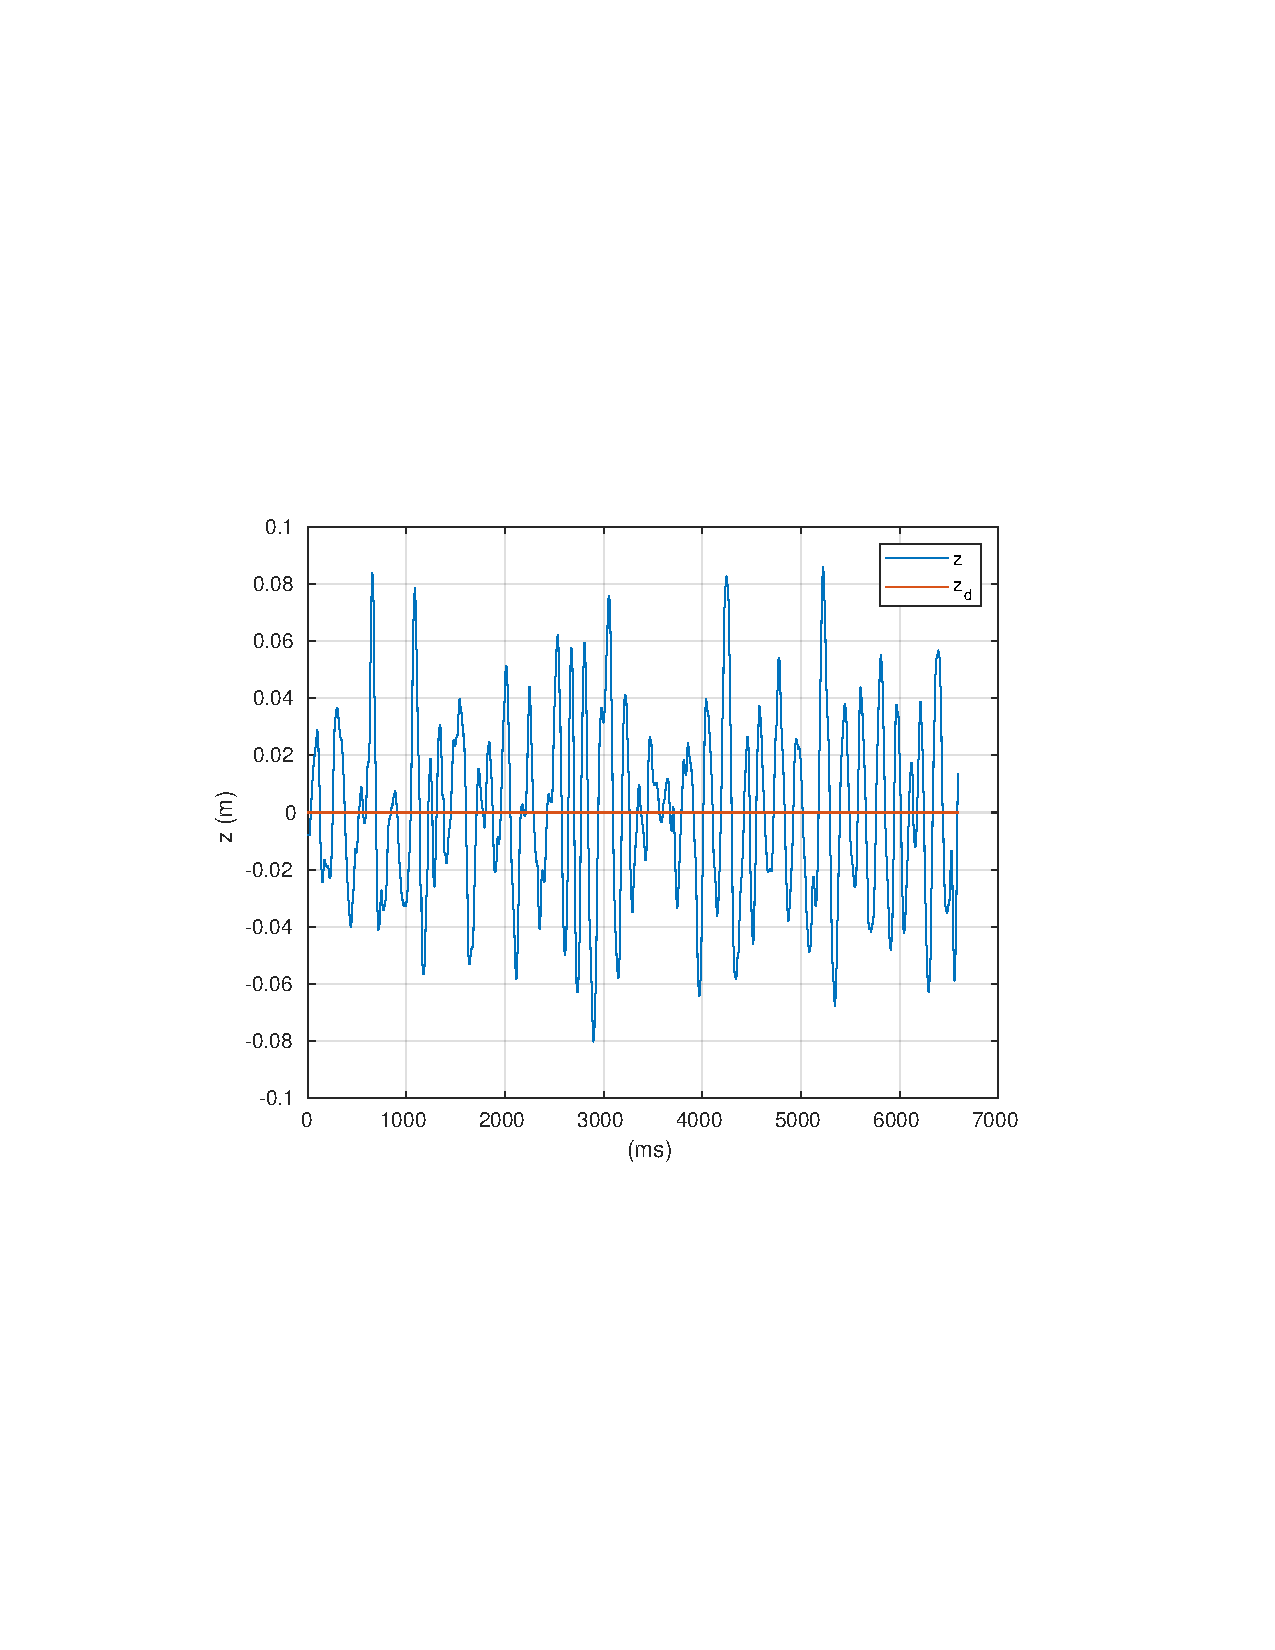
\includegraphics[scale=.7,trim={3.5cm 8cm 4cm 8cm},clip]{figuras/CROB_Fuzzy_Gerono/z.pdf}
		\caption{$z(t)$ for the Lemniscate of Gerono}
		\label{fig:crob_lem_z}
	\end{figure}
\end{frame}
%%%%%%%%%%%%%%%%%%%%%%%%%%%%%%%% FRAME %%%%%%%%%%%%%%%%%%%%%%%%%%%%%%%%
\begin{frame}
	\begin{figure}[!htb]
		% \includegraphics[trim={5cm 0 0 0},clip]{example-image-a}
		% 	 trim={<left> <lower> <right> <upper>}
		\centering
		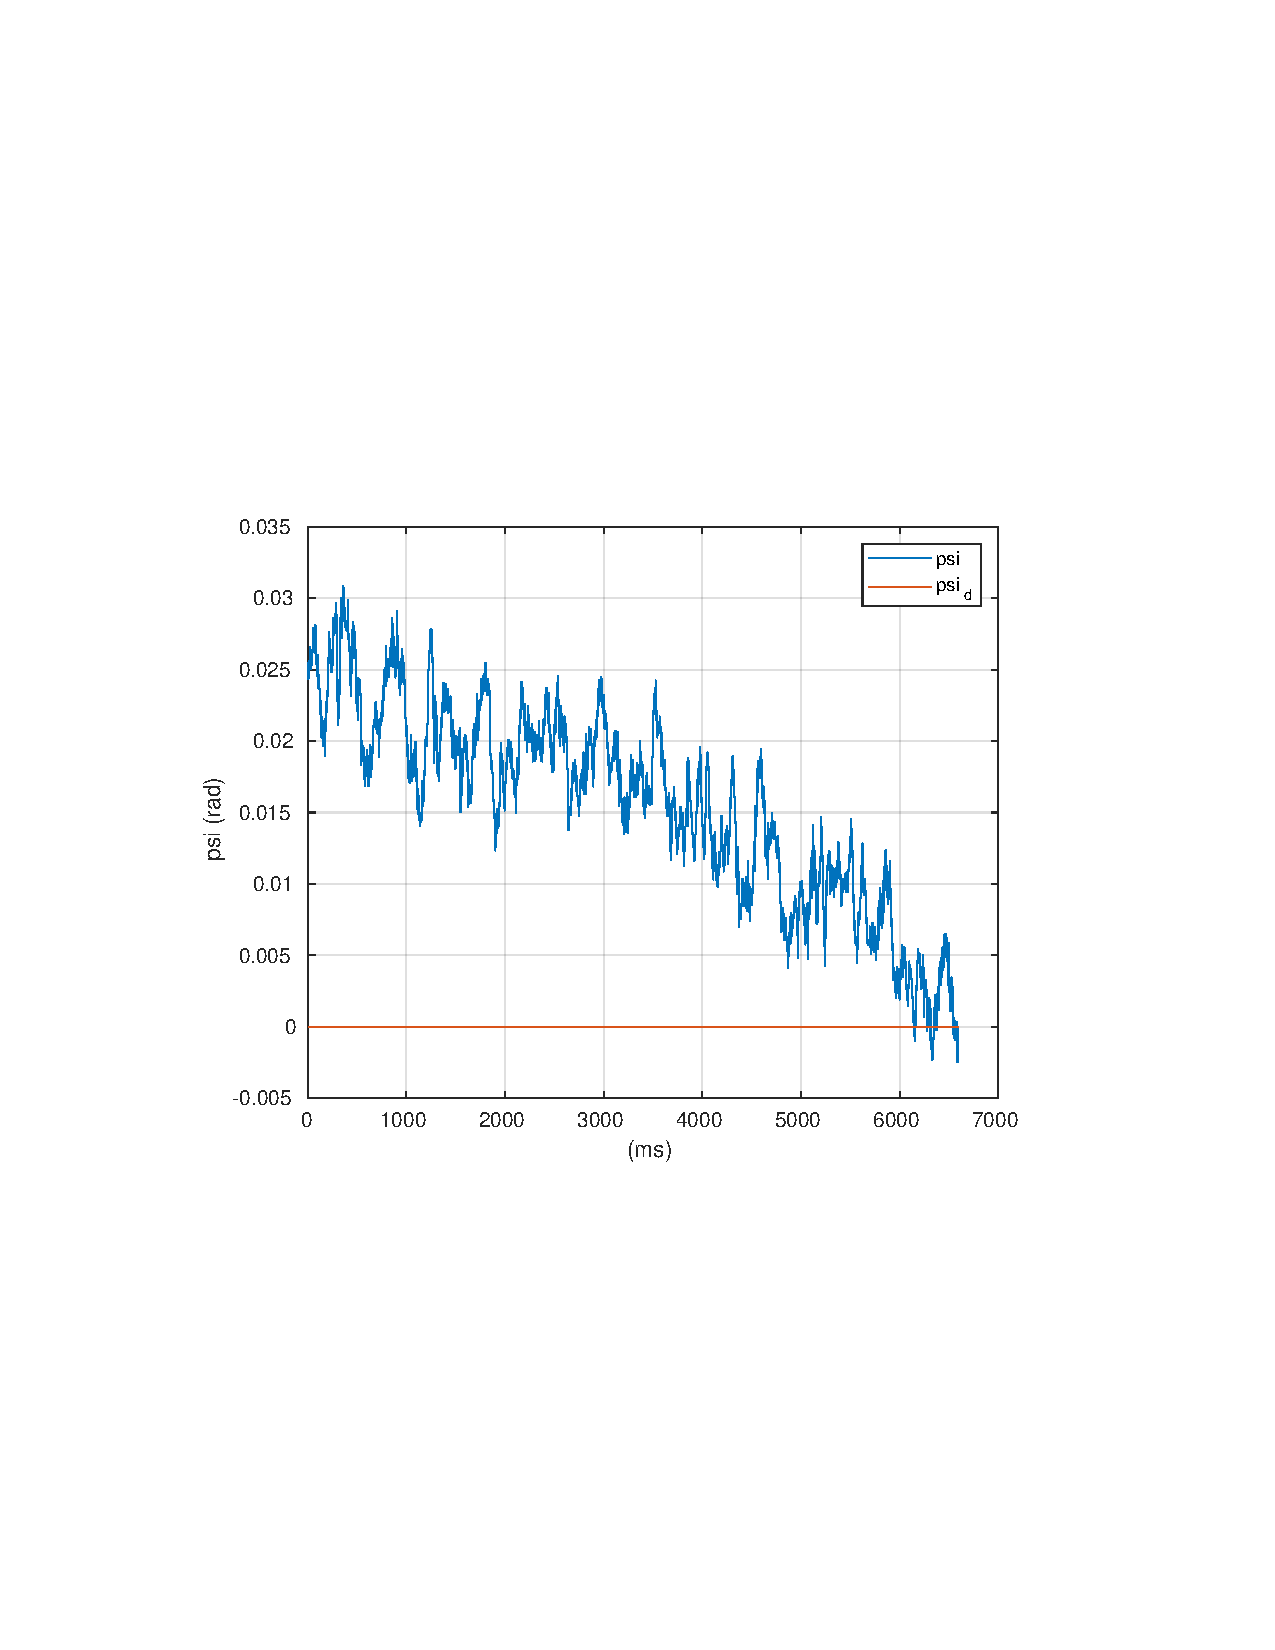
\includegraphics[scale=.7,trim={3.5cm 8cm 4cm 8cm},clip]{figuras/CROB_Fuzzy_Gerono/psi.pdf}
		\caption{$\psi(t)$ for the Lemniscate of Gerono}
		\label{fig:crob_lem_psi}
	\end{figure}
\end{frame}
%%%%%%%%%%%%%%%%%%%%%%%%%%%%%%%% FRAME %%%%%%%%%%%%%%%%%%%%%%%%%%%%%%%%
\begin{frame}{Results Overview}
	\begin{table}[h!]
		\centering
		\caption{Indoor Results}
		\begin{tabular}{||c c c c||} 
			\hline
			Trajectory & Mean (m) & standard deviation & \# of data points  \\ %[0.5ex] 
			\hline\hline
			\multirow{4}{*}{Circle} & $x:0.0681$ & $x:0.0394$ & \multirow{4}{*}{6303} \\
			& $y:0.0583$ & $y:0.0290$& \\
			& $z:0.0261$ & $z:0.0206$& \\
			& $\psi:0.0161$ & $\psi:0.0039$& \\ 
			& & & \\
			\multirow{4}{*}{Lemniscate} & $x:0.0470 $ & $x:0.0311$ & \multirow{4}{*}{6592} \\
			& $y:0.0717$ & $y:0.0372$& \\
			& $z:0.0260$ & $z:0.0185$& \\
			& $\psi:0.0156$ & $\psi:0.0070$& \\
			\hline
		\end{tabular}
		\label{table:indoor_res}
	\end{table}
	\end{frame}
%%%%%%%%%%%%%%%%%%%%%%%%%%%%%%%% FRAME %%%%%%%%%%%%%%%%%%%%%%%%%%%%%%%%